\chapter{Introduction and motivation}\label{cha:introduction_and_motivation}

\section{Outline of the problem}\label{sec:outline_of_the_problem}

Better camera calibration improves the performance of various downstream tasks
by providing a more accurate mapping between 3D world coordinates and 2D image
plane coordinates. This improved mapping enables precise alignment, positioning,
and scaling of objects within the scene. By determining the camera's intrinsic
and extrinsic parameters, algorithms can correct for lens distortion, estimate
depth information, and accurately overlay virtual content. Consequently, tasks
such as 3D reconstruction, augmented reality, and object detection can achieve
better results in terms of precision, spatial consistency, and overall visual
quality.

Although manufacturers can estimate camera calibration parameters a priori,
fully automatic calibration is often preferred, especially when camera metadata
is unavailable. Currently, wide-angle lenses, particularly in mobile phones and
GoPro-type cameras, dominate consumer photography. These cameras pose additional
challenges due to their requirement for highly non-linear models with numerous
parameters. The high distortion of the image plane also makes finding key points
robustly challenging.

Typically, camera calibration is obtained by capturing an image of a known
calibration pattern, which is then used to estimate the camera parameters.
Alternatively, some methods do not use a calibration pattern but instead infer
geometric constraints directly from the scene. However, this approach is
generally less accurate.

As reported by \textcite{duisterhofTartanCalibIterativeWideAngle2022} on
\citedate{duisterhofTartanCalibIterativeWideAngle2022}, the current state-of-the-art
methods
\citep{olsonAprilTagRobustFlexible2011, schopsWhyHaving102020,
	krogiusFlexibleLayoutsFiducial2019}
fail on images with high distortion.
\cite{duisterhofTartanCalibIterativeWideAngle2022} suggested an iterative
the approach of image undistortion and target reprojection, achieving the superior
robustness to the noise than the state-of-the-art methods because the feature
detection is performed on the undistorted image.
% \todo{Probably remove the emphasis on TartanCalib, if I am not going to compare
% with it}

Instead of searching for the features on the undistorted image from scratch, it
is possible to utilize the prior knowledge of the geometry of the calibration
board, effectively predicting the possible positions of previously undetected
features. It can be done by projecting the board onto the image using the
intermediate camera calibration, and then filtering the possible positions in
order to eliminate false positives.

This additional points will further constrain the camera calibration, improving
the accuracy of the calibration parameters.

\begin{figure}
	\begin{tikzpicture}[spy using outlines={circle,yellow,magnification=4,size=3cm, connect spies}]
		\node[anchor=south west,inner sep=0] (image) at (0,0)
    % {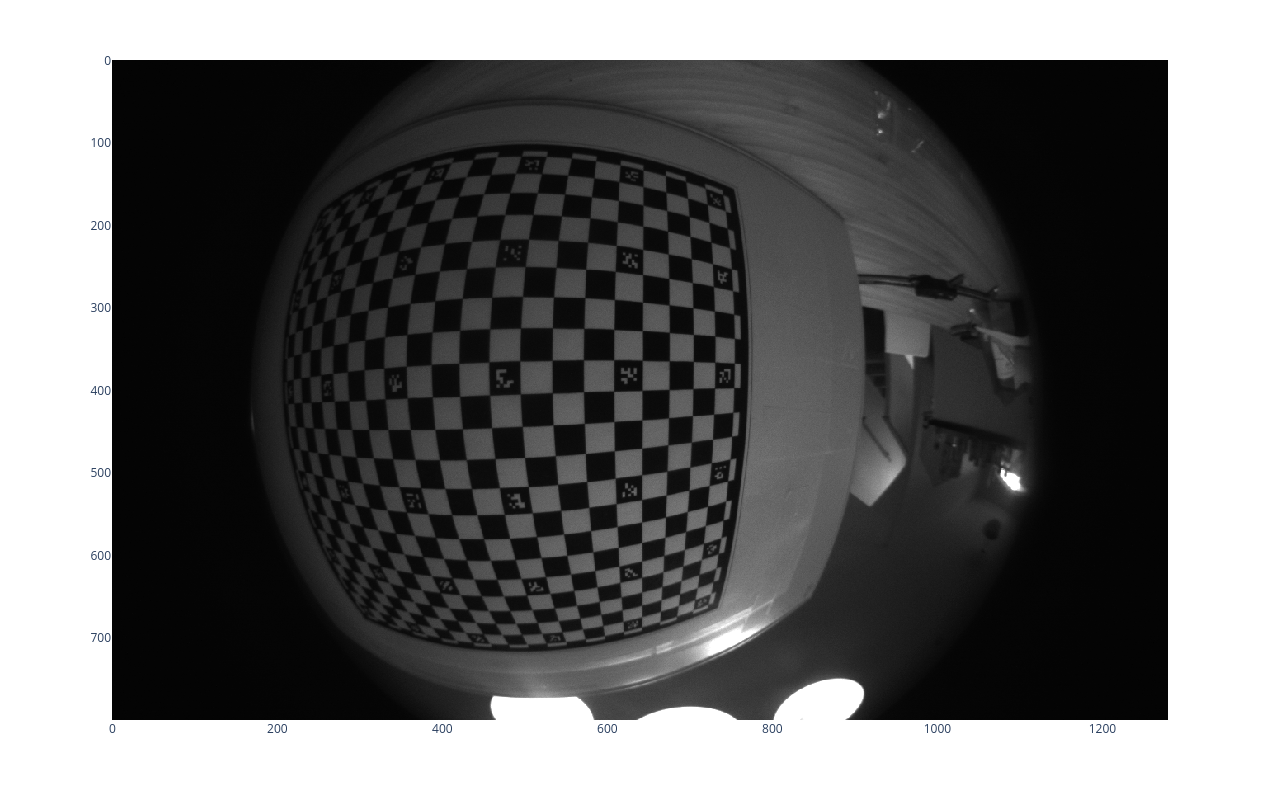
\includegraphics[width=0.6\textwidth]{distorted_image}};
    {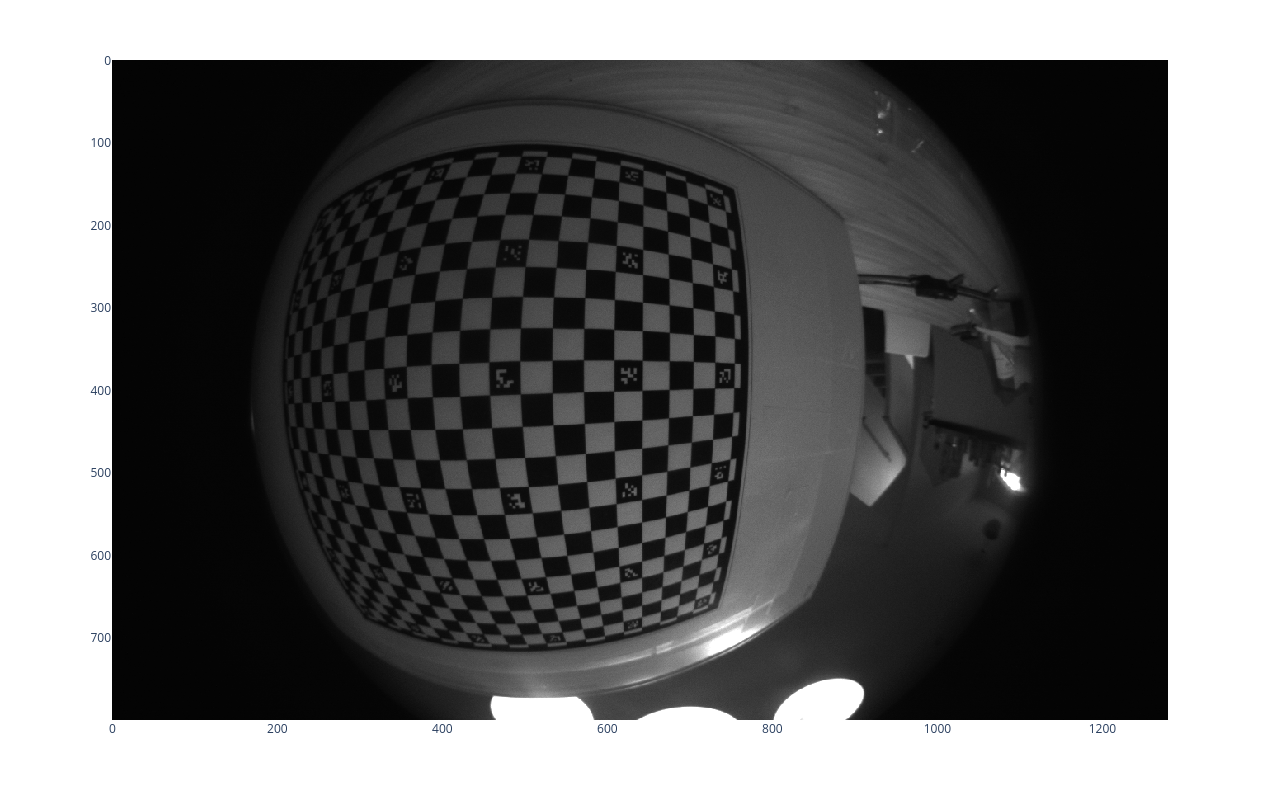
\includegraphics[width=0.8\textwidth]{distorted_image}};
		\begin{scope}[x={(image.south east)},y={(image.north west)}]
			\spy[red] on (3.3,1.7) in node [left] at (10.1,1.7);
			\spy[blue] on (4.6,3.2) in node [right] at (8.1,5.3);
		\end{scope}
	\end{tikzpicture}
  \caption{Example of corners near the center of the image and near the edge}
\end{figure}

\section{Research objective}\label{sec:research_objective}

The objective of this research is to improve the accuracy of the camera
calibration by finding previously undetected features on the calibration
board \todo{Probably rephrase if I won't compare the actual calibration}. For
that, we formulate the set of research questions:
\begin{itemize}
	\item How to find additional features on the calibration board which were not
	      detected by the feature detector?
	\item How to filter out falsely detected features?
	      \todo{Add more}
\end{itemize}

\section{Thesis structure}\label{sec:thesis_structure}

This paper has the following structure: in \autoref{sec:related_work}, we will describe the related work, including the
literature search method and methodology, various subtopics of the camera
calibration, mention conjugate translations, and outline the state-of-the-art
solutions. We define the research gap in \autoref{sec:gap_analysis} and outline
the proposed approach to solution and evaluation in
\autoref{sec:problem_setting_and_approach_to_solution}. We will describe the
early results in \autoref{sec:early_results_and_discussion}, including the
dataset analysis, feature detector, and conjugately translated points simulator.
In \autoref{sec:summary_and_future_work}, we will summarize the results and
outline future work.
\todo{Update}

\endinput


